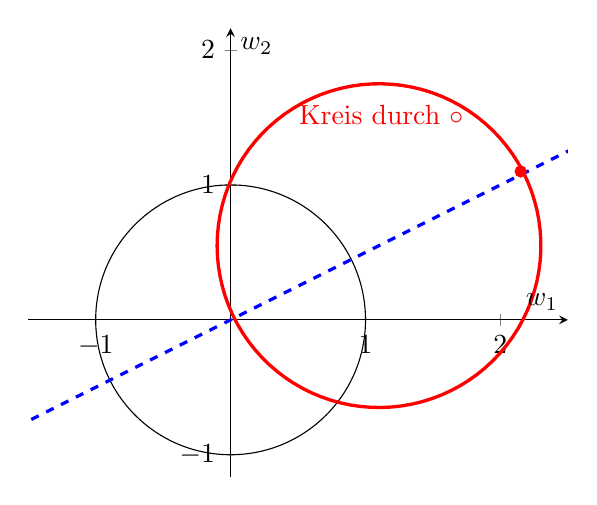
\begin{tikzpicture}
	\begin{axis}[
		axis lines=middle,
		axis equal,
		xmin=-1.5,
		xmax=2.5,
		ymin=-1,
		ymax=2,
		xlabel=$w_1$,
		ylabel=$w_2$,
	]	
		\draw (axis cs: 0, 0) circle [radius=1];
		\addplot[domain=-180:180, samples=100, color=red, very thick] ({1.2*cos(x) + 1.1}, {1.2*sin(x) + 0.55}) node[above, left, red, pos=0.65] {Kreis durch $\circ$};
		\addplot[-, blue, very thick, dashed] {0.5*x};
		\addplot[mark=*, red] coordinates {(2.15, 1.1)};
	\end{axis}
\end{tikzpicture}